\documentclass{article}

\usepackage{graphicx}
\usepackage[colorlinks=true, allcolors=blue]{hyperref}
\usepackage{float}
\usepackage{subcaption}
\usepackage{multirow}

\title{Linear Regression versus Random Forest Regression for House Prices in California \\[1ex] \large Project Report}
\author{Jeremiah Hawkinson \\ ID: 006002668}
\date{December 2022}

\graphicspath{{Images/}}

\begin{document}

\maketitle

%TC:ignore
\begin{center}
    
\includegraphics[scale=0.22]{Images/college logo.png}

    \vspace{0.8cm}

    School of Computer Science\\
    California State University San Bernardino\\

    \vspace{0.8cm}

    \textit{Professor} Yan Zhang

    \vspace{0.8cm}

\end{center}

\pagebreak

\begin{abstract}
Linear Regression and Random Forest Regression are two well known machine learning algorithms. In this report they are both tested and compared on a medium data set of California house prices by district from a 1990 census to see which of the algorithms performs best in predicting a house's price. The data was scaled using standardization, null values were filled using the median of its own attribute, and unnecessary attributes were dropped to best suit our prediction algorithms. The base parameters of the sklearn library for python was used to complete these tests. It was discovered that Random Forest Regression is superior at predicting the price of a house in California.
\end{abstract}

\section{Introduction}

There are many machine learning algorithms available for us to use. In this paper we will be testing the effectiveness of Linear Regression and Random Forest Regression in predicting house prices of California as shown in a \href{https://www.kaggle.com/datasets/camnugent/california-housing-prices?datasetId=5227}{1990 census}, found from the database of \href{https://www.kaggle.com/}{Kaggle}. They will be tested using the same data and compared to each other to determine which machine learning algorithm does the best job in predicting the prices of houses in California.

\section{Machine Learning Algorithms}

\subsection{Linear Regression}

Linear regression analysis is used to predict the value of one variable based on other variables. The variable you want to predict is called the dependent variable. The variable(s) you are using to predict the other variable's value is called the independent variable.

\begin{figure}[H]
\centering
\includegraphics[width=8.0cm]{LinearRegression_Example.png}
\caption{\label{fig:LinearRegression_Example}\href{https://data-science-blog.com/blog/2022/05/02/understanding-linear-regression-with-all-statistical-terms/}{Example of Linear Regression.}}
\end{figure}

Linear Regression estimates the coefficients of the linear equation, involving one or more independent variables to predict the value of the dependent variable. It fits a straight line or surface that minimizes the discrepancies between predicted and actual output values. A simple linear regression calculator uses a “least squares” method to discover the best-fit line for a set of paired data. You then estimate the value of x (dependent variable) from y (independent variable).

\subsection{Random Forest Regression}

Random Forest Regression is a type of classification that uses a large number of decision trees that work together as an ensemble. It uses bagging and feature randomness when building each individual tree to try to create an uncorrelated forest of trees, then uses averaging to increase predictive accuracy and help control over-fitting of the data set.

\begin{figure}[H]
\centering
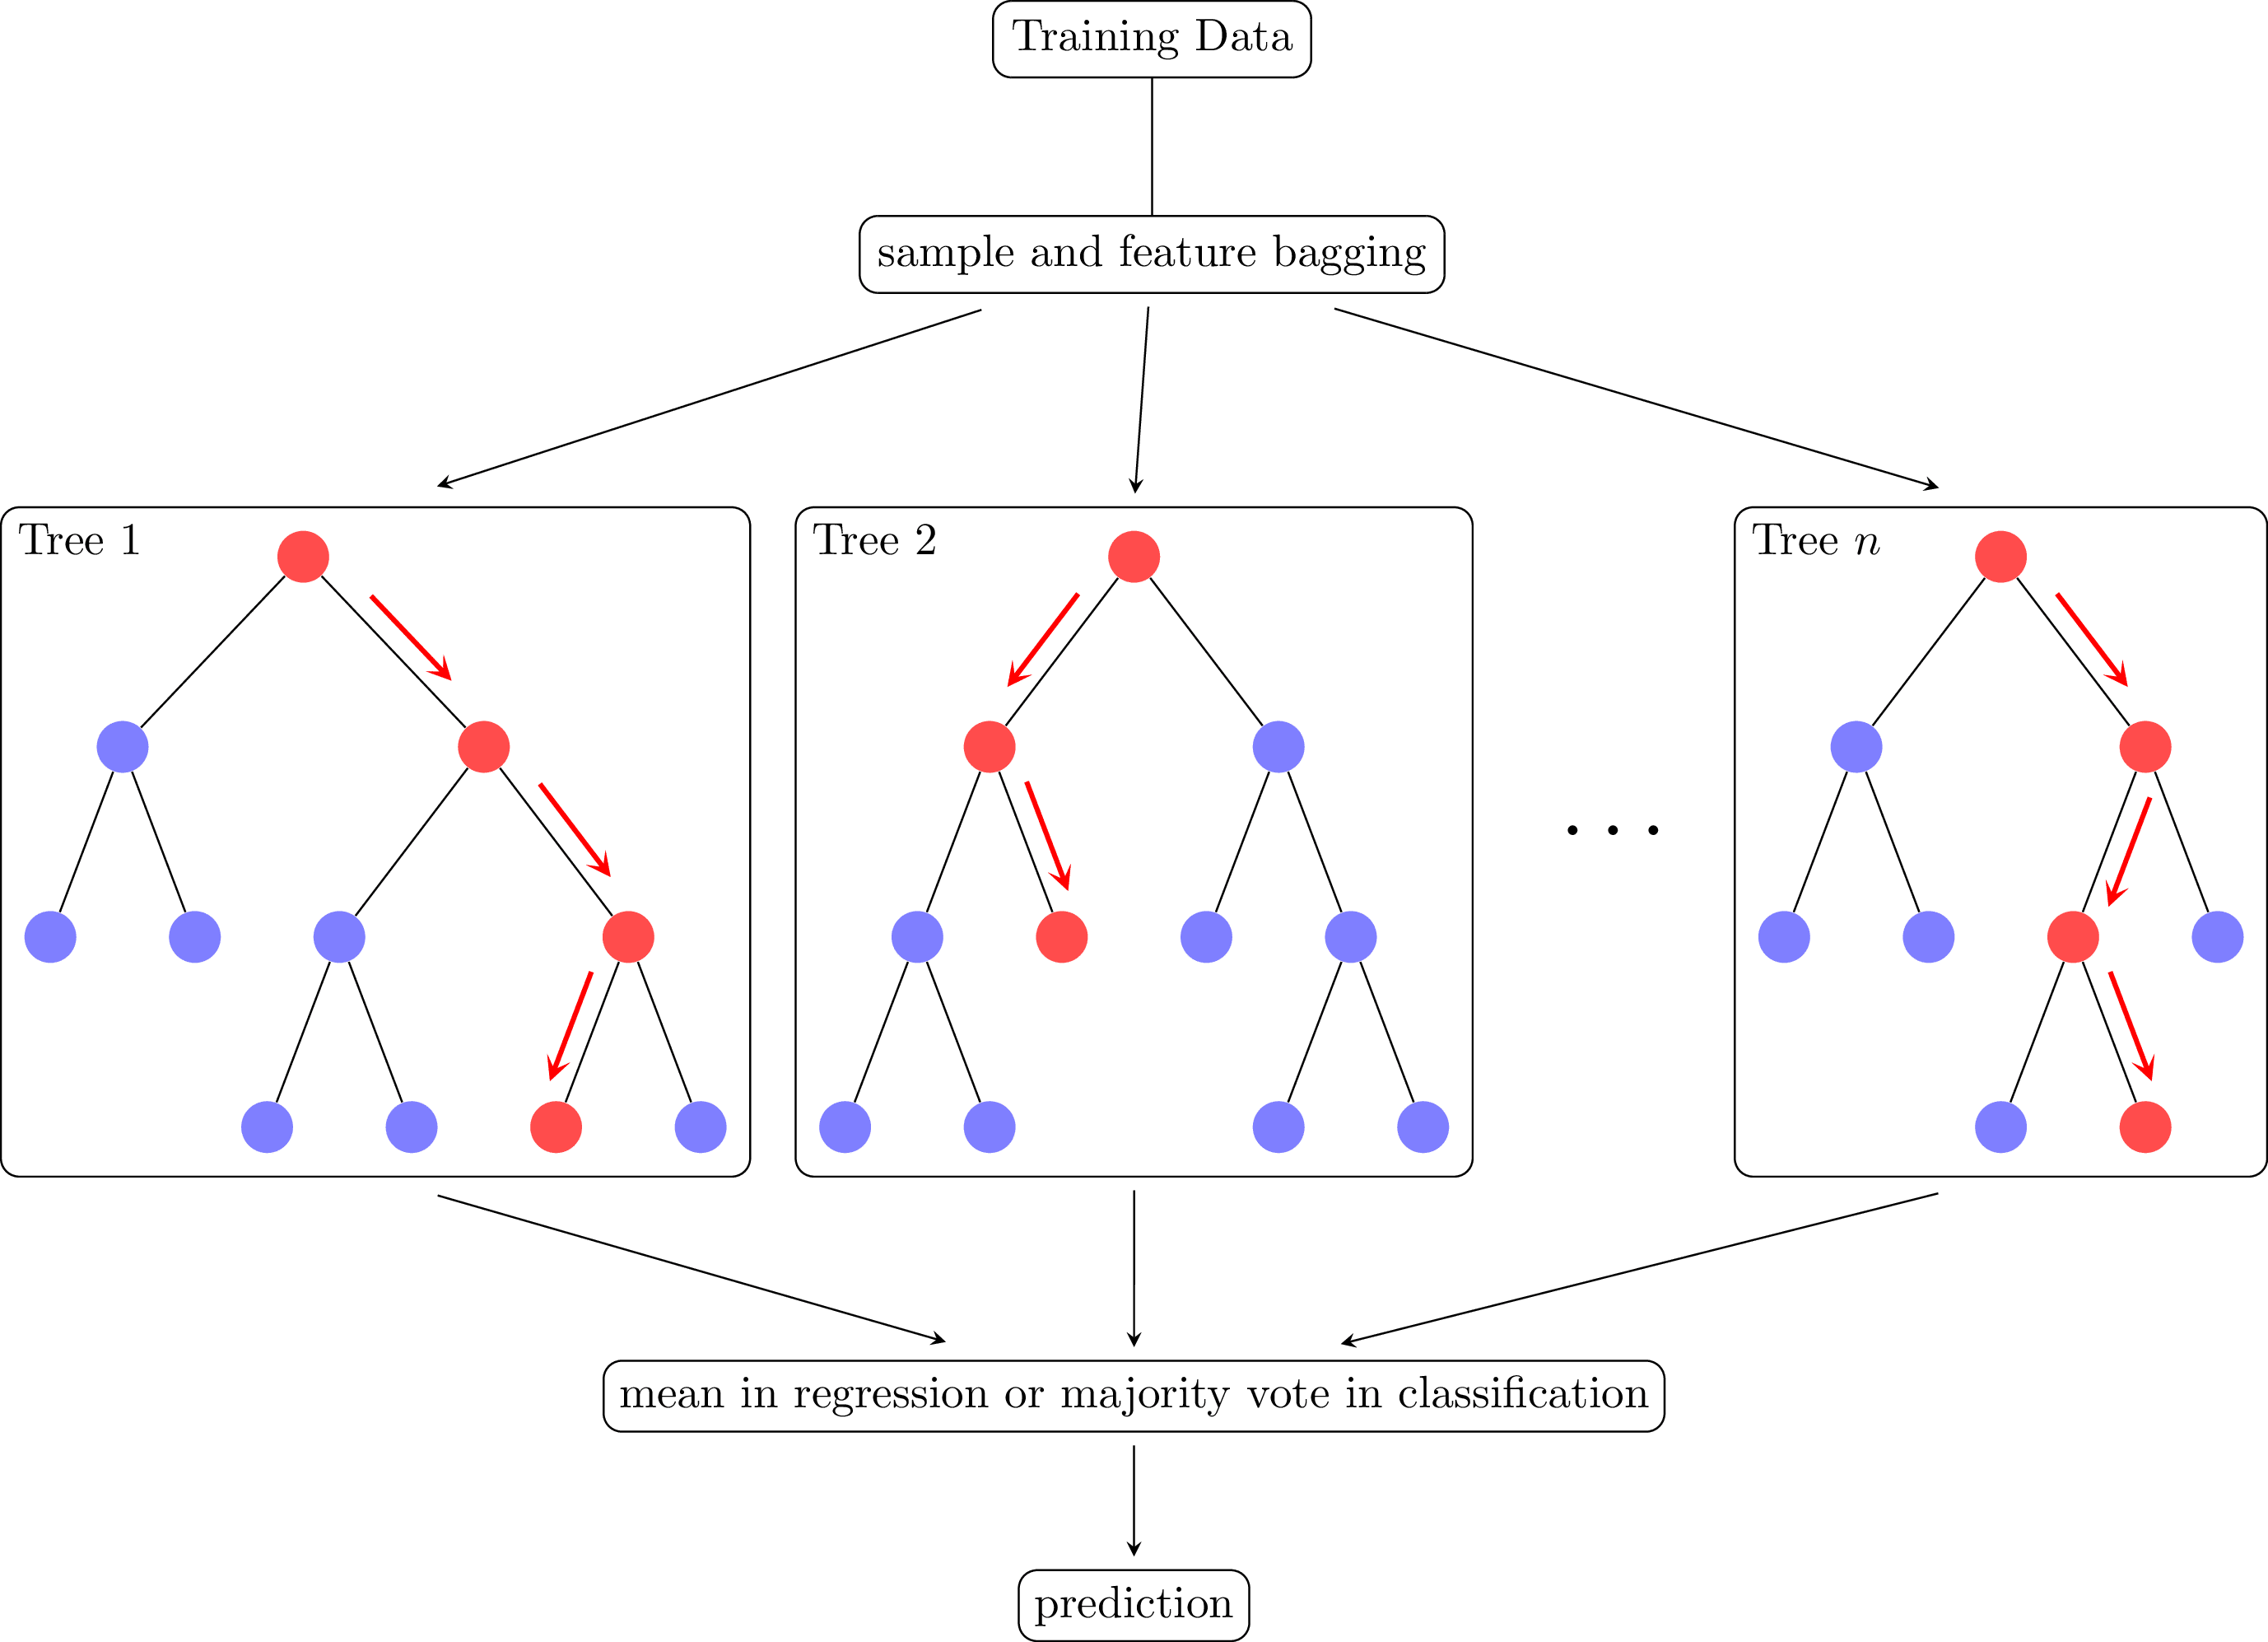
\includegraphics[width=12.0cm]{random-forest.png}
\caption{\label{fig:random-forest}\href{https://tikz.net/random-forest/}{Example of a Random Forest decision trees.}}
\end{figure}

\section{Data Set and Experiment}

\subsection{Data Set: California Housing Prices}

The data set includes the information for house prices for California districts derived from a 1990 census.

\begin{figure}[H]
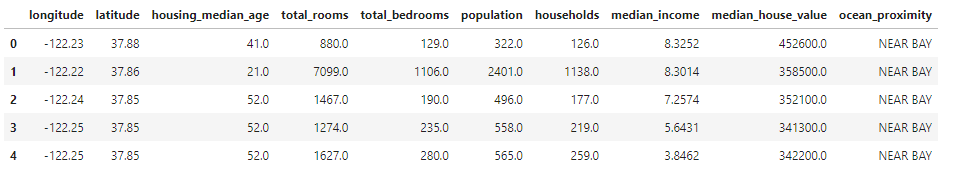
\includegraphics[width=15.0cm]{Images/dataset_columns.png}
\caption{\label{fig:dataset_columns}Header of the California House Prices Data Set}
\end{figure}

\begin{figure}[H]
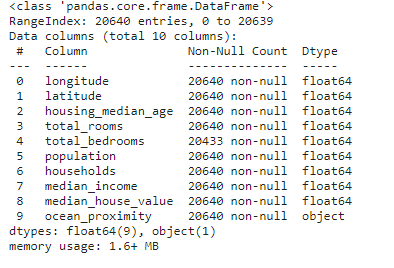
\includegraphics[width=9.0cm]{Images/housing_info.png}
\caption{\label{fig:housing_info}Information on the columns and data types of the data set.}
\end{figure}

There are 10 columns in the data set and 20640 entries for us to test. Small grievances such as the "ocean proximity" column being a categorical object instead of numerical will require us to decide on an approach method to prepare the full data set for testing. Another issue shown in Figure~\ref{fig:housing_info} shows that the column "total bedrooms" has 207 null values that also need to be addressed before testing.

\subsection{Correlation Matrix and Feature Engineering}

Using the correlation matrix it is possible to determine what attributes have the largest affinity with the attribute that is trying to be predicted. In this case "Median House Value" is the attribute which is being predicted.

\begin{figure}[H]
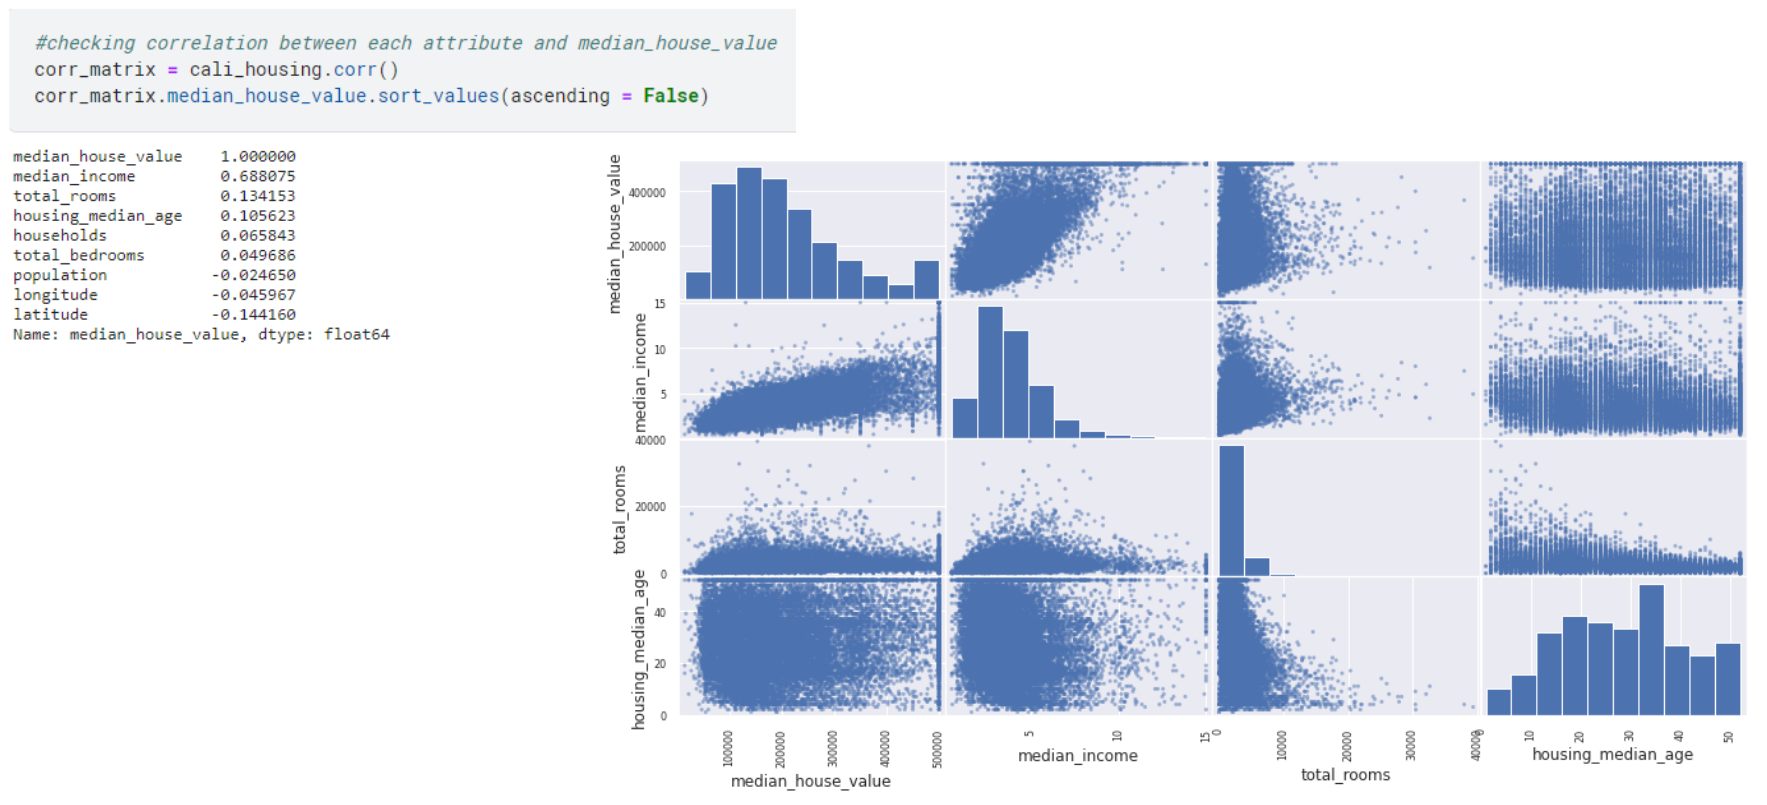
\includegraphics[width=12.5cm]{Images/correlation histogram.png}
\caption{\label{fig:correlation histogram}Histogram of the top four correlated attributes.}
\end{figure}

Seeing how "total rooms" is valued so highly in correlation to the value of a house, a step further can be taken to possibly increase the rate of our prediction by adding some new feature attributes. Using the attributes "total rooms" and "households" we can find out the number of rooms per household in a district to help better represent our data. Another attribute that was created was "people per household" using the "population" and "household attributes. These added attributes can be seen in the correlation matrix of Figure~\ref{fig:new_correlation}

\begin{figure}[H]
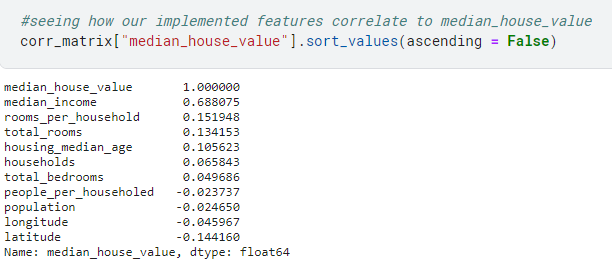
\includegraphics[width=10.0cm]{Images/new_correlation.png}
\caption{\label{fig:new_correlation}New attribute "rooms per household" is third in correlation.}
\end{figure}

\subsection{Data Preprocessing}

Moving back to the small grievances stated in Section 3.1. It was necessary to fix the null values within attribute "total bedrooms". This was done by using the sklearn simple imputing function of python to get the median of each attribute and filled any null values within the data set using them. The categorical value of "ocean proximity" was dropped from the data set as it would contribute little to overall prediction of house values and could not be used as a non-numerical value.

The range of the data in each value varies greatly in this data set so it is necessary to scale it. The data was scaled using standardization, and the attributes were split into "x" and "y" to prepare it for our machine learning algorithms. For our Linear Regression algorithm the "median household value" was dropped and put into "y" while the other attributes were called into "x" to fuel our prediction. The last instance of data preprocessing was splitting our data set into a train and test set using the sklearn library. There is a test set of 20 percent, numbering 4,128 instances, and a training set of 80 percent, numbering 16,512 instances.

\begin{figure}[H]
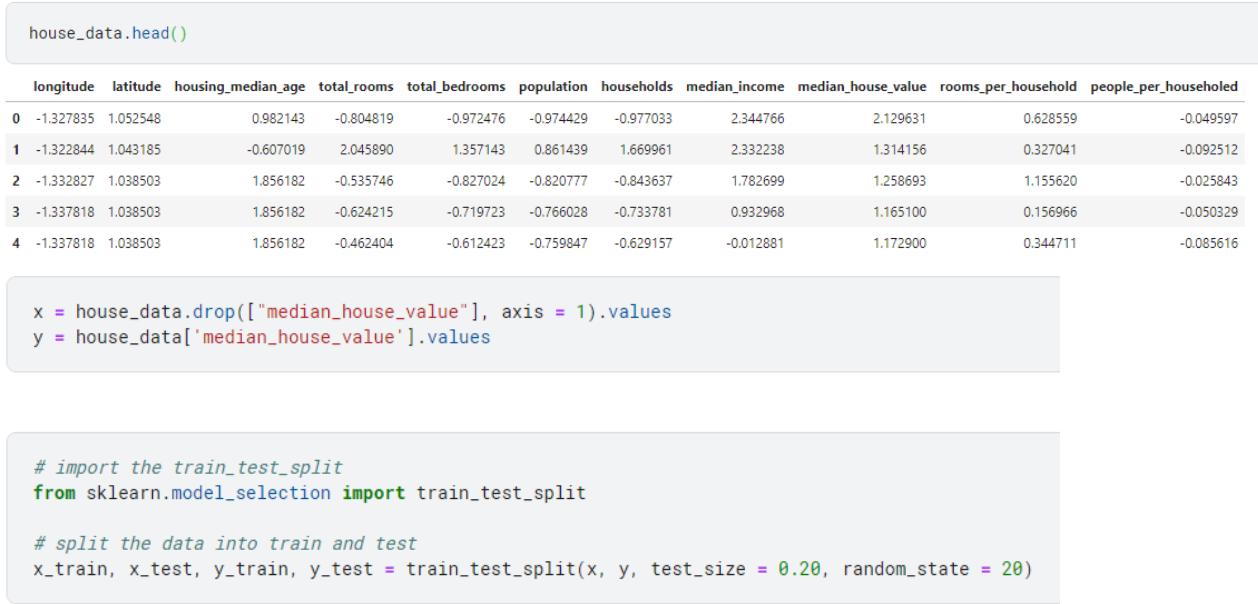
\includegraphics[width=13.0cm]{Images/preprocessing.png}
\caption{\label{fig:preprocessing}Scaled data and training/test sets.}
\end{figure}

\subsection{Algorithm Parameters}
The parameters used for the machine learning algorithms in our experiment were both the base parameters given by the imported library sklearn. A random state of 20 was given as a parameter to each for easier replication of the experiment. Random Forest Regression used n = 100 for its estimation.

\section{Evaluation and Comparison}

\subsection{Linear Regression}

The Linear Regression test score achieved by our machine algorithm managed to reach 62.7 percent using our test size and reached 63.9 percent with our training set as seen in Figure~\ref{fig:linear_regression}. The coefficients from the training and test sets are shown and a comparison of the predicted values versus actual values are shown in Figure~\ref{fig:linreg_comparisonI} The root mean squared error came out to 0.6248 which is acceptable given the complexity of the data set and our scores for Linear Regression.

\begin{figure}[H]
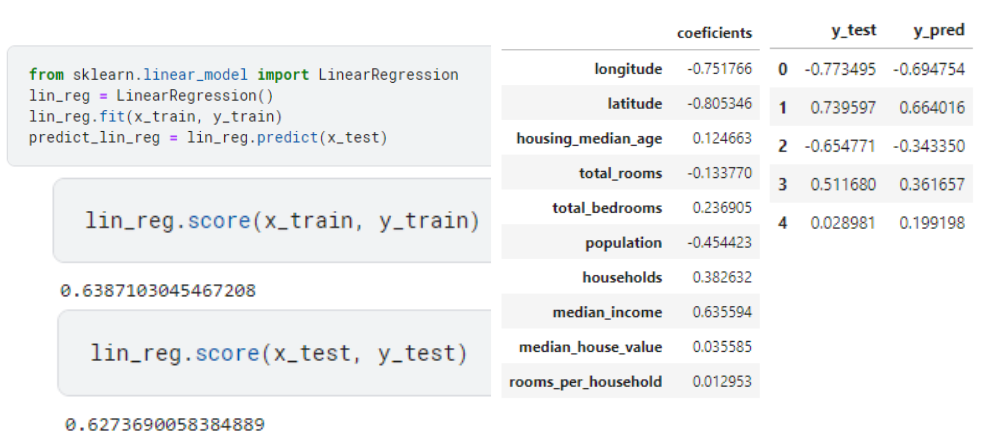
\includegraphics[width=13.0cm]{Images/linear_regression.png}
\caption{\label{fig:linear_regression}Scores for the training and test sets. Linear Regression coefficients for predicted results and actual results.}
\end{figure}

\begin{figure}[H]
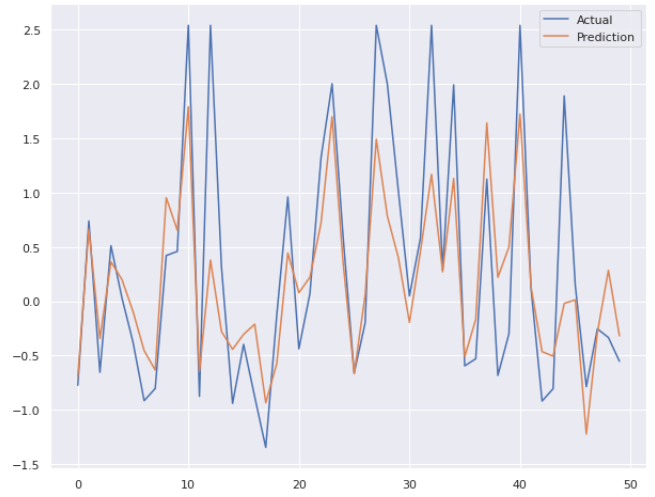
\includegraphics[width=11.0cm]{Images/linreg_comparisonI.png}
\caption{\label{fig:linreg_comparisonI}Actual values versus predicted values.}
\end{figure}

\subsection{Random Forest Regression}

The Random Forest Regression algorithm was ran using base sklearn parameters with n=100 for estimators and random state=20. This gave a large improvement over the Linear Regression scores with an 81.5 percent using the test set and a 97.3 percent using the training set. The root mean squared error was also minimally 0.4396 showing considerable results. 

\begin{figure}[H]
\centering
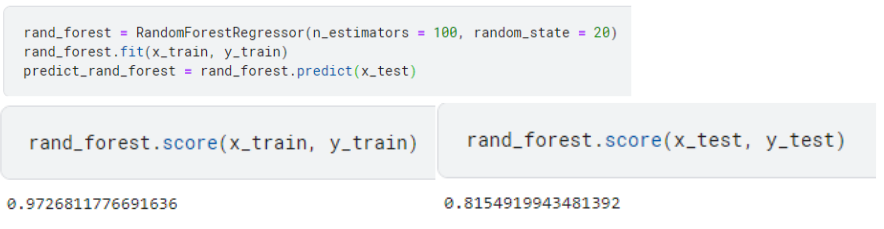
\includegraphics[width=12.0cm]{Images/rand_forest_score.png}
\caption{\label{fig:rand_forest_score}Scores for the Random Forest Regression algorithm.}
\end{figure}

\subsection{Comparison}

Random Forest Regression performed considerably better than Linear Regression in predicting the median house value of houses in California using our data set. Obtaining accurate results 19 percent more often, and at a lower margin of error.

\begin{tabular}{ |c|c|c|c| } 
\hline
 & R$^2$ Score & Root Mean Squared Error \\
\hline
Random Forest & 0.815492 & 0.439649 \\ 
\hline
Linear Regression & 0.627369 & 0.624796 \\ 
\hline
\end{tabular}

\section{Conclusion}

In conclusion Random Forest Regression is significantly better at predicting the house prices of California using this data set than Linear Regression. Random Forest Regression had a 81.5 percent chance of correctly predicting while Linear Regression achieved a 62.7 percent chance. Both of these test are sufficient in attempting to predict something as complex as the housing market of California but Random Forest Regression does it more effectively.

\bibliography{sample}

\end{document}